\section{Durchführung}\label{sec:durchfuehrung}
In diesem Kapitel werden die Szenarien im Detail beschrieben, sowie deren Paketmittschnitte analysiert.

\subsection{Echo Dot}
Ziel der Analyse des Echo Dot ist es zum Einen zu ermitteln, mit welchen Servern das Gerät kommuniziert.
Außerdem soll untersucht werden, ob tastächlich erst dann Sprachdaten übertragen werden, wenn das Aktivierungswort genannt wird.

\subsubsection{Einschalten}
Schaltet man den Echo Dot ein, so leuchtet der LED-Ring blau auf und ein hellblauer Balken rotiert.
Damit wird signalisiert, dass der Echo zwar eingeschaltet ist, allerdings kann er keine Befehle entgegennehmen,
da er gerade einen anderen Prozess ausführt.
Was dies im konkreten Fall des Einschaltens ist, wird im Folgenden analysiert.

\begin{figure}[h!]
    \centering
    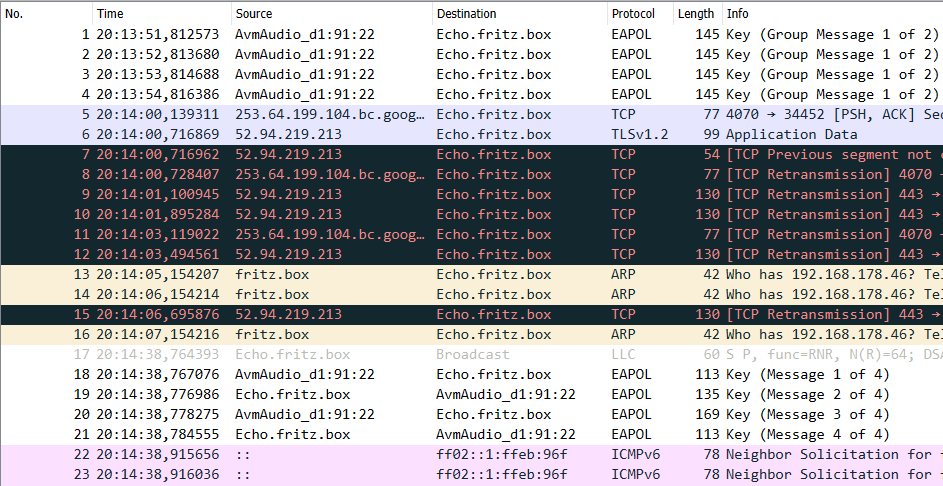
\includegraphics[width=\textwidth]{echoEin/start}
    \caption{Erste Pakete beim Einschalten des Echo Dot}\label{fig:echo-ein-start}
\end{figure}

\paragraph{Verbindungsaufbau}
Der Paketmittschnitt beginnt mit verschiedenen Paketen, welche an den Echo Dot gesendet werden (siehe \autoref{fig:echo-ein-start}).
Darunter befinden sich auch mehrere ARP-Requests ausgehend vom Router.
Da diese unbeantwortet bleiben kann davon ausgegangen werden, dass der Echo Dot zu diesem Zeitpunkt noch nicht in Betrieb ist.
Diese Vermutung wird dadurch gestützt,
dass in den darauffolgenden Paketen 17 bis 21 der 4-Wege-Handshake \cite[S.~169f]{Bless2006} nach IEEE 802.11i durchgeführt wird.

\begin{figure}[ht!]
    \centering
    \resizebox{0.75\textwidth}{!}{
        \input{assets/uml/WPA2.latex}
    }
    \caption{IEEE 802.11i 4-Wege-Handshake}
    \label{fig:handshake}
\end{figure}

Der Handshake wird mit einer Authenitfizierunganfrage (17) gestartet.
Die Pakete 18 und 19 dienen dem Austausch von Nonces zwischen den beiden Geräten.
Ab Paket 19 wird mit jedem Paket ein \ac{mic} gesendet, um die Intregrität der Nachrichten zu sichern.

Zur späteren Verschlüsselung der Nachrichten zwischen den beiden Geräten wird der \ac{ptk} genutzt.
Er leitet sich ab aus dem \ac{pmk}, den beiden Nonces sowie den MAC-Adressen der beiden Geräte.
Der \ac{pmk} ist ein beiden Geräten bekannter Schlüssel, welcher im Voraus verteilt wurde.
In diesem Fall handelt es sich um den \enquote{WLAN-Netzwerkschlüssel}.

Der \ac{ptk} kann lediglich für direkte Verbindungen zwischen den beiden Geräten verwendet werden (Unicast).
Um auch Multi- und Broadcast Nachrichten zu untertützen wird in Paket 20 ein \ac{gtk} gesendet.
Dieser ist mehreren Teilnehmern bekannt und kann so für Multicast-Nachrichten verwendet werden.


\paragraph{Übersicht Verbindungen}
Nach dem Verbindungsaufbau wird über das DHCP-Protokoll eine IP-Addresse erfragt und zugeteilt.
Darauf folgen von Echo Dot ausgehend verschiedene DNS-Anfragen, welche vom Router beantwortet werden.
Erhält der Echo Dot eine solche Antwort, so wird eine TCP-Verbindung zu dem Server aufgebaut.
Häufig diese Verbindung durch TLSv1.2 verschlüsselt. In diesen Fällen kann der Inhalt der Pakete nicht analysiert werden.

Es werden Verbindungen zu folgenden Servern aufgebaut:

\begin{table}[ht!]
    \centering
    \begin{tabular}{|l|r|}
        \hline
        \textbf{Server} & \textbf{Verschlüsselt} \\
        \hline
        kindle-time.amazon.com & Nein \\
        \hline
        pindorama-eu.amazon.com & Ja \\
        \hline
        dp-gw-na.amazon.com & Ja \\
        \hline
        dcape-na.amazon.com & Ja \\
        \hline
        s3-1-w.amazonaws.com & Nein \\
        \hline
        prod.amcs-tachyon.com & Ja \\
        \hline
        www.example.com & Nein \\
        \hline
        www.example.org & Nein \\
        \hline
        weblb-wg.dual-gslb.spotify.com & Nein \\
        \hline
        gew1-accesspoint-b-ttcq.ap.spotify.com & Nicht durch TLS \\
        \hline
        device-messaging-na.amazon.com & Ja \\
        \hline
        todo-ta-g7g.amazon.com & Ja \\
        \hline
        arcus-uswest.amazon.com & Ja \\
        \hline
        updates.amazon.com & Ja \\
        \hline
    \end{tabular}
    \caption{Verbindungen des Echo Dot beim Einschalten}
    \label{tab:verbindungenEchoDot}
\end{table}




Aus den nicht verschlüsselten Verbindungen lassen sich folgende Informationen ermitteln:

\subparagraph{kindle-time.amazon.com}
Dieser Server wird zwei Mal während des Einschaltvorgangs angesprochen.
Beide Male ist dies ein HTTP-Request direkt an die URL \url{http://kindle-time.amazon.com/}.
Als Antwort liefert der Server in beiden Fällen den Fehlercode \texttt{403 Forbidden}.
Aus der Subdomain \textit{kindle-time} kann geschlossen werden,
dass die Anfrage zum Ermitteln der aktuellen Uhrzeit gedacht ist.

Da die Antwort mit dem Fehlercode ein \texttt{Date}-Feld enthält,
erfüllt die Abfrage eventuell auf diesem Weg ihren Zweck.
\begin{figure}[h!]
    \centering
    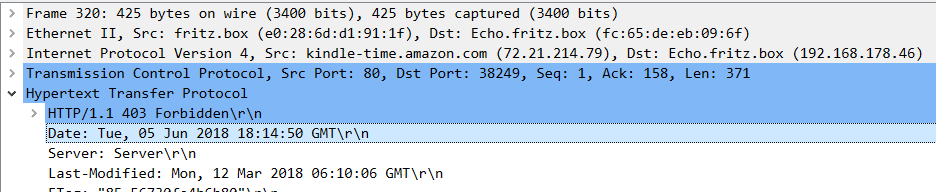
\includegraphics[width=\textwidth]{echoEin/kindle-time}
    \caption{Antwort von kindle-time.amazon.com mit Date-Feld}\label{fig:echo-ein-start}
\end{figure}


\subparagraph{s3-1-w.amazonaws.com}
Auch dieser Server wird zweimal über HTTP angesprochen.
Die entsprechende URL lautet \url{http://spectrum.s3.amazonaws.com/kindle-wifi/wifistub-echo.html}.
Als Antwort liefert der Server eine HTML-Seite,
welche lediglich den Text \texttt{81ce4465-7167-4dcb-835b-dcc9e44c112a} enthält.

Zwar gibt es keine offiziellen Informationen zum Nutzen dieser Nachricht.
Vermutlich handelt es sich hierbei um einen Weg Amazon mitzuteilen,
dass das Gerät online ist.


\subparagraph{www.example.com, www.example.org}
Bei diesen beiden Servern handelt es sich um Server der Organisation IANA (Internet Assigned Numbers Authority).
Die Server und zugehörigen URLs dienen als Beispiele in Dokumenten \cite{IANA:online}.
In dem Paketmittschnitt wird zu \url{www.example.com} eine TCP-Verbindung über IPv6
und zu \url{www.example.org} eine TCP-Verbindung über IPv4 aufgebaut und direkt wieder geschlossen.

Da verschiedene IP-Versionen genutzt werden, hat es den Anschein,
dass getestet werden soll über welche Version eine Verbindung ins Internet möglich ist.

\subparagraph{weblb-wg.dual-gslb.spotify.com}
Dieser Server gehört zum bekannten Musik-Steamingdienst Spotify.
Eine Verbindung wird Aufgebaut, da der Echo Dot dort als Wiedergabegerät hinterlegt ist.
Der Server wird mit zwei URLs jeweils über HTTP angesprochen.
Die erste URL lautet \url{http://esdk-ffl.spotify.com/esdk-fire-and-forget/} und enthält die zwei Parameter \texttt{key\_id=1} und \texttt{value}.
Der zweite Parameter ist eine lange Folge von Buchstaben, Zahlen und Sonderzeichen.
Als Antwort liefert der Server hier lediglich den Statuscode \texttt{200 OK} ohne weitere Daten.

Die zweite URL (\url{http://apresolve.spotify.com/?client=2:5:0:71778584372445291}) liefert Daten im JSON-Format als Antwort.


\lstinputlisting[
    caption=Antwort von apresolve.spotify.com,
    label=lst:spotify,
    language=json
]{spotify.json}

Die Antwort ist eine Liste von URLs von \enquote{Access Points}.
Der Echo Dot verbindet sich im weiteren Verlauf mit dem ersten dieser Access Points.


\subparagraph{gew1-accesspoint-b-ttcq.ap.spotify.com}
Die TCP-Verbindung zu diesem Server ist zwar nicht mittels TLS verschlüsselt,
allerdings werden auch keine Daten im Klartext übertragen.
Somit handelt es sich entweder um anderweitig verschlüsselte Daten oder
um in einem nicht lesbaren Format verpackte Anwendungsdaten.\\

Alle anderen Verbindungen verben mittels TLSv1.2 verschlüsselt.
Daher kann der Inhalt der Pakete nicht (in Klartext) betrachtet werden.
Lediglich aus den Metadaten wie \textit{Server-Adresse} oder \textit{Paketgröße} können Annahmen über den Zweck der Verbindung getroffen werden.


Aus den Verbindungen zu den Servern
\url{pindorama-eu.amazon.com},
\url{dp-gw-na.amazon.com},
\url{dcape-na.amazon.com},
\url{prod.amcs-tachyon.com},
\url{device-messaging-na.amazon.com},
\url{todo-ta-g7g.amazon.com} und
\url{arcus-uswest.amazon.com}
können keine Informationen ermittelt werden.
Auch eine Recherche bleibt erfolglos.

Lediglich aus der Verbindung \url{updates.amazon.com} kann aufgrund ihrer Subdomain geschlossen werden,
dass durch diesen Server geprüft wird, ob ein Update der Software des Echo Dot verfügbar ist.

\todo[inline]{Zwischenfazit?}

\subsubsection{5 Minuten reiner Netzverkehr (keine Befehle)}
Amazon behauptet, dass der Echo Dot keine Sprachpakete ohne konkreten Befehl des Nutzers an Server zur verarbeitung sendet.
Dem entgegen stehen Berichte in welchen behauptet wird das Gerät \enquote{schneidet heimlich [ein] Gespräch mit}\cite{AmazonEc81:online}.
Hierbei handelt es sich jedoch nicht um \enquote{heimliches} Mitschneiden. Es wurden in dem Gespräch lediglich Aussagen in der Weise missverstanden,
dass diese als Befehl aufgefasst wurden.

Ob der Echo Dot auch im Ruhezustand Daten sendet und wenn ja an wen und was für Daten soll in diesem Abschnitt untersucht werden.

Der Paketmittschnitt zeigt Verbindungen zu Servern welche bereits bei Start des Echo Dot kontaktiert wurden.
Zu den Servern \url{www.example.com} und \url{s3-1-w.amazonaws.com} wird vermutlich eine Verbindung aufgebaut um dein Oline-Status des Echo Dot zu prüfen und diesen an Amazon mitzuteilen.
Außerdem wird eine Verbindung zu dem bereits bekannten Server \url{dp-gw-na.amazon.com} hergestellt.

Zusätzlich werden auch neue Server angesprochen:
\begin{description}
    \item[222.64.199.104.bc.googleusercontent.com]
        Diese Adresse verweist auf einen Server der von \textit{Google Cloud Platform} gehosted wird.
        Da diese Plattform von jedem genutzt werden kann und die TCP-Verbindung verschlüsselt ist,
        kann über den Zweck der Verbindung keine Aussage getroffen werden.
    \item[ntp-g7g.amazon.com]
        Der Server hinter dieser Adresse wird über das \ac{ntp} angesprochen.
        Das Protokoll dient zur Synchronisation der Uhrzeit über das Netzwerk.
    \item[ec2-34-196-73-245.compute-1.amazonaws.com]
        Hierbei handelt es sich um eine \textit{Amazon Elastic Compute Cloud}\cite{WasistAm39:online}.
        Für diesen Server gilt wie bereits für den \textit{Google Cloud Platform}-Server,
        dass jeder einen solchen Server mieten kann.
        Hierdurch und durch die ebenfalls verschlüsselte Verbindung kann auch hier keine Aussage über den Zweck getroffen werden.
    \item[*.amazonaws.com (52.216.100.3)]
        Der letze neu hinzugekommene Server wird über die IP-Adresse \texttt{52.216.100.3} angesprochen.
        Der Name dieses Servers kann nicht aufgelöst werden, da die DNS Anfrage bereits vor dem Start der Aufzeichnung stattfand.
        Eine Recherche zeigt jedoch, dass auch diese Adresse teil der \textit{Amazon Web Services} ist.
        Interessant an den Paketen ist,
        dass das beim ersten aufgezeichneten TCP-Paket,
        welches vom Echo Dot an den Server gesendet wird,
        das \texttt{FIN}-Flag gesetzt ist.
        Hierdurch wird signalisiert, dass die Verbindung beendet werden soll.
        Daraufhin werden neun identische Pakete mit den \texttt{RST}-Flag gesendet.
        Ein solches Flag wird in der Regel dann gesendet, wenn eine TCP-Verbindung nicht möglich ist.
        Der Echo Dot beantwortet die identischen Pakete, in dem er die Fehlermeldung \textit{TCP Retransmission} an den Server sendet.
        Möglicherweise wurde die Verbindung zwischen den Partnern nicht erfolgreich geschlossen, was zu diesen Fehlern führte.
        \begin{figure}[h!]
            \centering
            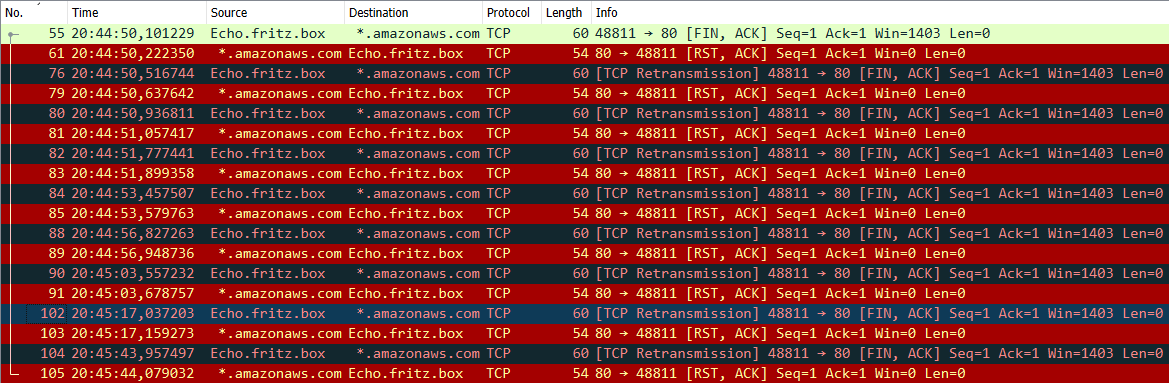
\includegraphics[width=\textwidth]{echoEin/echo-fehler}
            \caption{Identische Pakete mit RST-Flag und TCP Retransmission-Meldung}\label{fig:echo-fehler}
        \end{figure}
\end{description}

Der Paketmittschnitt belegt, dass der Echo Dot auch im Ruhezustand mit Servern im Internet kommuniziert.
Vor allem durch die sehr allgemeinen Kommunikationspartner der \textit{Google Cloud Platform} und der \textit{Amazon Elastic Compute Cloud}
kann der Zweck dieser Verbindungen nicht immer bestimmt werden.
Betrachtet man jedoch die Größe der gesendeten Pakete, so ist festzustellen,
dass lediglich zwei Pakete größer als 100 Bytes sind.
Das eine Paket ist ein HTTP-GET-Request mit 200 Bytes an \url{s3-1-w.amazonaws.com} und
das andere ein TLSv1.2-Paket mit 295 Bytes an \url{dp-gw-na.amazon.com}.

Bezieht man nun noch mit ein, dass vom Echo Dot innnerhalb der fünf Minuten nur 66 Pakete gesendet wurden,
dann kann davon ausgegangen werden, dass in dieser Zeit keine Sprachoakete gesendet wurden.

\subsubsection{Erfragen des aktuellen Wetters}
\todo[inline]{Weglassen, weil keine wirkliche Online-Verarbeitung gezeit wird?\\Oder besser so was wie Nachrichten?}


\subsection{Playstation 4}
Wie bereits in Kapitel \ref{sec:aufbau} \textit{\nameref{sec:aufbau}} gezeigt, wird die Playstation 4 über verschiedene Kanäle angesteuert.
Anhand des Ein- und Ausschaltens soll der kommunikationstechnische unterschied dieser Kanäle untersucht werden.

\subsubsection{Ein- und Ausschalten über \textit{Hassbian}}
\textit{Hassbian} bzw. der darin installierte Home Assistant bieten zur Steurung der konfigurierten Geräte eine Weboberfläche.
In \autoref{fig:hass-ui} ist der Schalter hervorgehoben, welcher für das Ein- und Ausschalten der Playstation 4 genutzt wird.

\begin{figure}[h!]
    \centering
    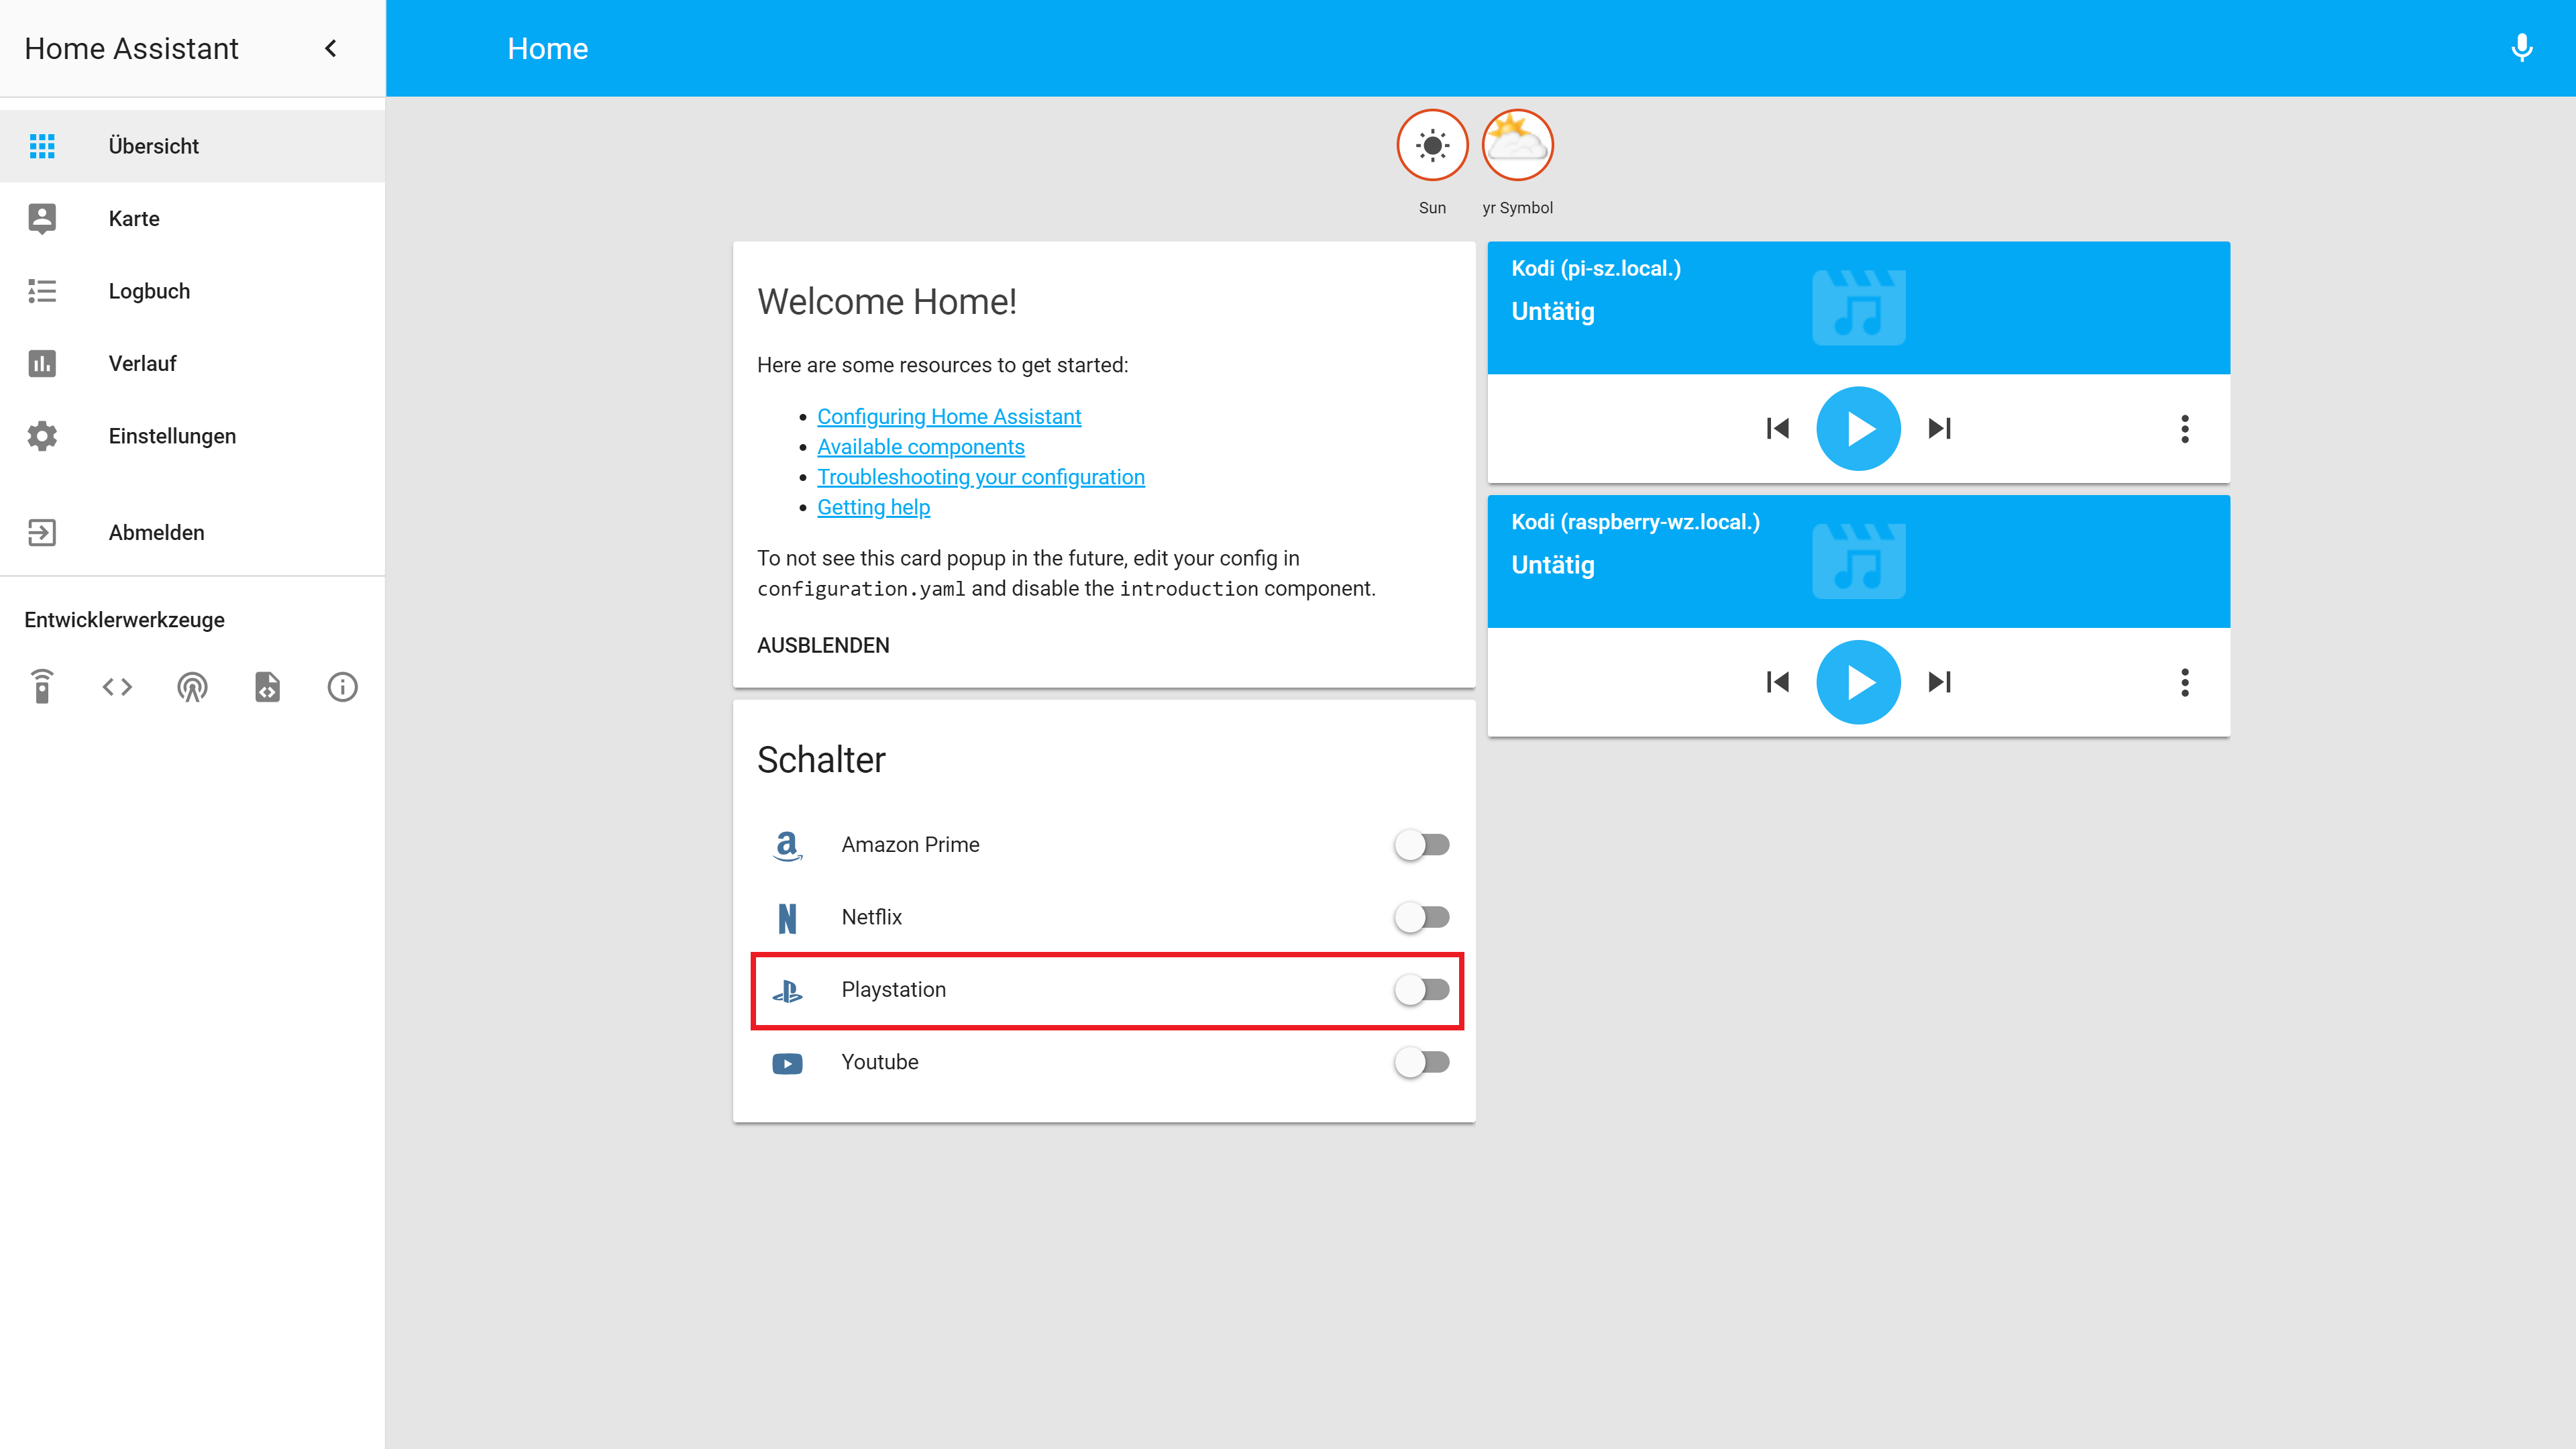
\includegraphics[width=\textwidth]{hass_ui}
    \caption{Weboberfläche des Home Assistant}\label{fig:hass-ui}
\end{figure}

Zum Einschalten wird der Befehl \texttt{ps4-waker -d 192.168.178.34 \\ -c \textasciitilde{}/.homeassistant/.ps4-wake.credentials.json} über das \ac{cli} abgesetzt.
Der Befehl weist das Programm \textit{ps4-waker} dazu an sich mit der Playstation 4 unter der IP-Adresse \texttt{192.168.178.34} zu verbinden und dabei die Zugangsdaten in der angegebenen JSON-Datei zu nutzen.

Das Ausschalten folgt nach einem ähnlichen Muster.
In dem Befehl wird noch das Kommando \texttt{standby} angehängt,
um die Playstation 4 auszuschalten (bzw. in den Ruhezustand zu versetzen). \\

Auch anhand der jeweiligen Paketmittschnitte ist ein gemeinsames Muster zu erkennen.
Der jeweilige Befehl wird mittels einer TCP-Verbindung Ausgeführt
während parallel mehrere UDP-Pakete in beide Richtungen gesendet werden.
Hierbei kommunizieren die beiden Geräte direkt miteinander.

Laut dem Entwickler dienen die UDP dazu, zu prüfen, ob die \ac{ps4} bereit ist eine Verbindung anzunehmen.
Hierzu werden zunächst zwei UDP-Pakete mit den in \autoref{lst:ps4-wakeup} gezeigten Daten
und dann ein UDP-Paket mit in \autoref{lst:ps4-launch} gezeigten Daten.
Das Feld \texttt{user-credential} (in den Listings gekürzt) ist hierbei immer gleich
und wurde beim Initialen Verbindungsaufbau ermittelt.

\lstinputlisting[
    caption=Daten eines WAKEUP-Paketes,
    label=lst:ps4-wakeup
]{ps4_wakeup.udp}

\lstinputlisting[
    caption=Daten eines LAUNCH-Paketes,
    label=lst:ps4-launch
]{ps4_launch.udp}

Der eigentliche Befehl wird dann in der auf die UDP-Pakete folgenden TCP-Verbindung ausgeführt.
Zwar ist diese Verbindung nicht mit TLS verschlüsselt, die Daten können dennoch nicht ausgelesen werden.
Die Ursache hierfür ist im Quellcode des \textit{ps4-waker} ersichtlich.
Die Daten werden dort vor dem Senden auf Anwendungsebene verschlüsselt.

\subsubsection{Ein- und Ausschalten über \textit{Harmony Hub}}
Im Harmony Hub ist zur Nutzung der Playstation 4 eine Aktion konfiguriert.
Neben dem Ein- und Ausschalten der \ac{ps4} selbst wird auch der Fernseher eingeschaltet und der entsprechende Eingangskanal gewählt.

Zum Einschalten wird der durch den Home Assistant bereitgestelle Schalter genutzt. Über die emulierte \textit{Hue Bridge} erscheint dieser als Lampe im Harmony Hub.

Ist die \ac{ps4} eingeschaltet, so kann der Hub eine Bluetooth-Verbindung aufbauen. Daher ist es zum Ausschalten nicht nötig den Home Assistant zu nutzen.
Der Hub schlatet die Konsole direkt über die Bluetooth-Verbindung aus, sobald die Aktion beendet wird.

\subsubsection{Ein- und Ausschalten über \textit{Echo Dot}}
Das Ein- bzw. Ausschalten der Playstation über den Echo Dot fügt dem Prozess eine weitere Abstraktionssutfe hinzu.
Der entsprechende Befehl hierzu lautet \enquote{Alexa, schalte Playstation ein (bzw. aus) mit Harmony}.
Mit dem Suffix \enquote{mit Harmony} wird der Echo Dot dazu angewiesen den Befehl an den Harmony-Skill weiterzuleiten,
welcher wiederum den Harmony Hub anspricht.


\subsection{Kodi}
\todo[inline]{Überleitung warum noch Kodi Betrachtet wird (im sinne von Professionell vs Konfigurierbar)}

Das folgende Kapitel betrachtet die Steuerung von \textit{Kodi} über die offizielle Smartphone-App \textit{Kore}.
Eine Steuerung über den Harmony Hub ist auch möglich.
Allerdings erfolgt diese über Bluetooth und wird daher im Rahmen dieses Projektes nicht betrachtet.

\subsubsection{Navigieren mit Pfeiltasten in der Smartphone-App}
\textit{Kore} ermöglicht es mit Pfeiltasten innerhalb von \textit{Kodi} zu navigieren.
Anhand dieses Beispiels soll die grundlegende Kokmmnunikation zwischen \textit{Kore} und \textit{Kodi} gezeigt werden.

\begin{figure}[h!]
    \centering
    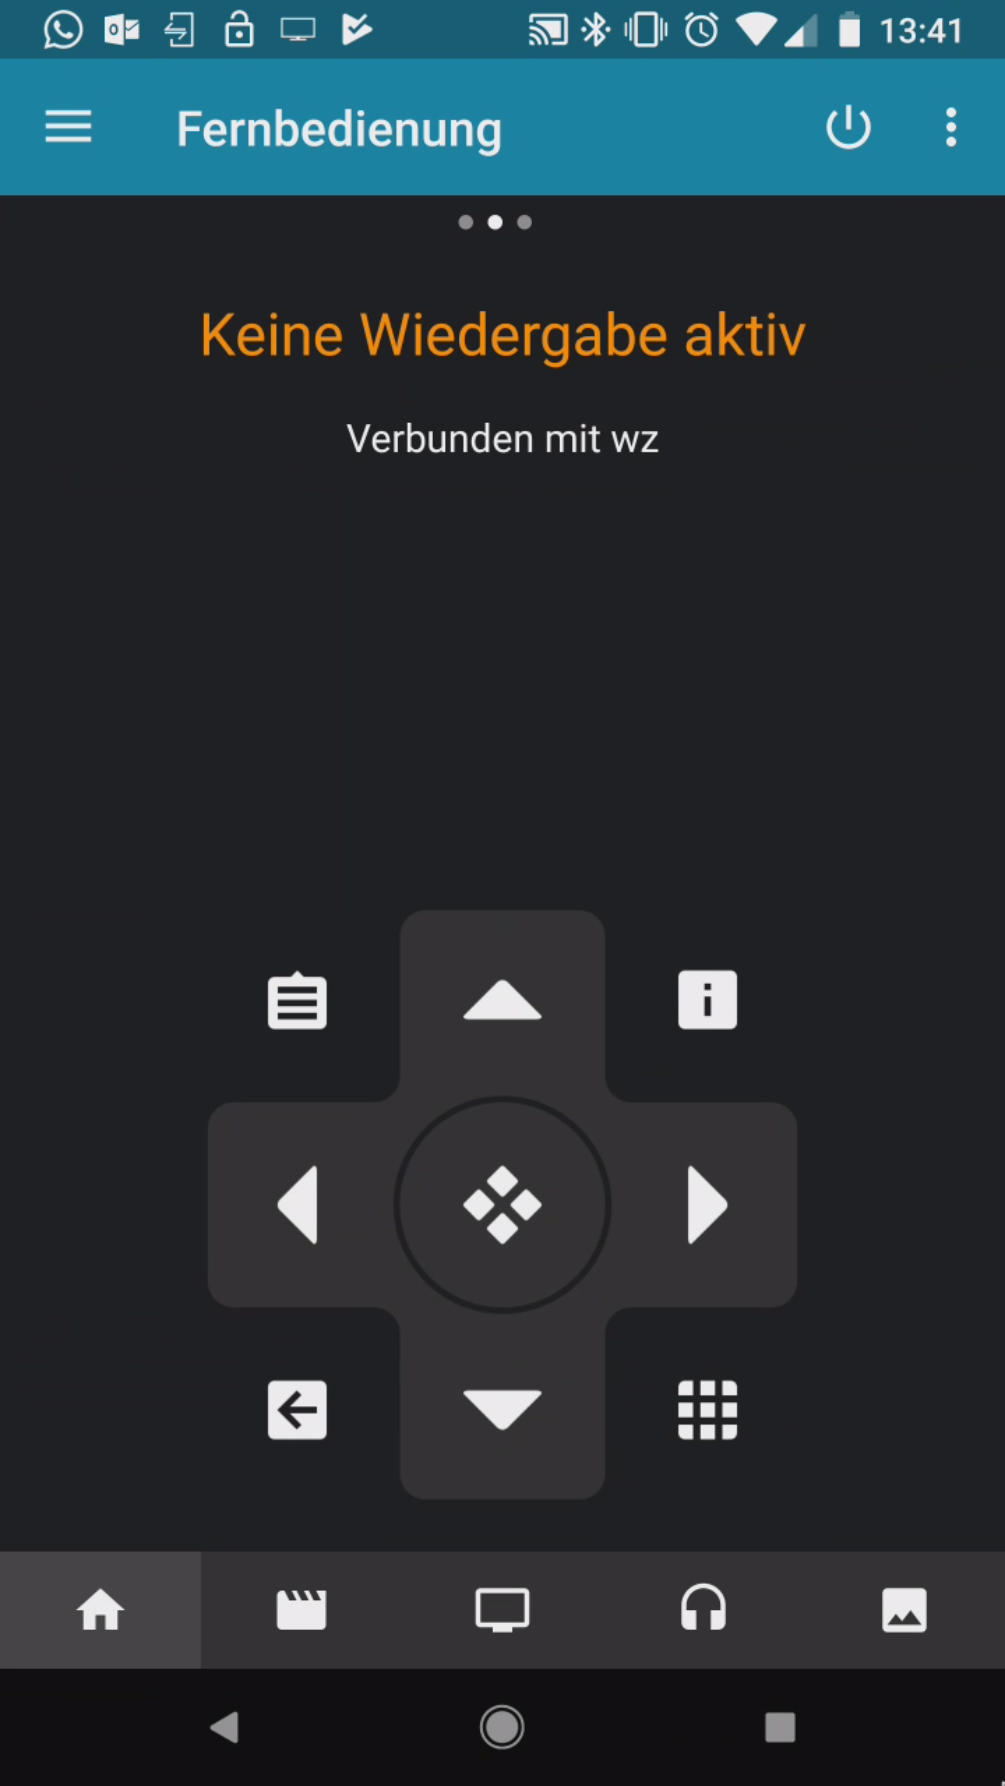
\includegraphics[width=0.5\textwidth]{kore}
    \caption{Oberfläche von Kore}\label{fig:kore}
\end{figure}


\subsubsection{Kurzes Fernsehen gesteuert von der Smartphone-App}
Das letze zu Betrachtende Szenario ist ein beispielhaftes Fernsehen über \textit{Kodi}.
Es beginnt mit dem Auswählen des Senders,
daraufhin wird die Lautstärke angepasst und zum Schluss wird die Wiedergabe beendet.